\documentclass[12pt,a4paper]{article}
\usepackage[utf8]{inputenc}
\usepackage[portuguese]{babel}
\usepackage[margin=2.5cm]{geometry}
\usepackage{url}
\usepackage{amsmath}
\usepackage{amsfonts}
\usepackage{amssymb}
\usepackage{graphicx}

\title{MAC0344 Arquitetura de Computadores\\Lista de Exercícios No. 2}
\author{Aluno: Leonardo Heidi Almeida Murakami \\ NUSP: 11260186}
\date{\today}

\begin{document}

\maketitle

\section*{Questão 1}

\begin{figure}[h!]
    \centering
    \begin{minipage}{0.48\textwidth}
        \centering
        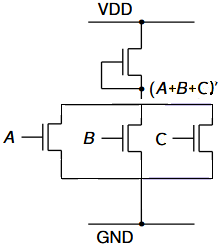
\includegraphics[width=\textwidth]{NOR_3INPUT.png}
        \caption{(a) Porta NOR com 3 entradas.}
    \end{minipage}
    \hfill
    \begin{minipage}{0.48\textwidth}
        \centering
        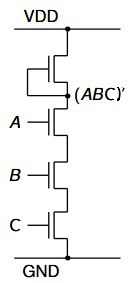
\includegraphics[width=0.75\textwidth]{NAND_3INPUT.png}
        \caption{(b) Porta NAND com 3 entradas.}
    \end{minipage}
\end{figure}

\newpage
\section*{Questão 2}

A alternativa correta é a \textbf{(b)}.

A resistência efetiva de condução ($r_{ef}$) de um transistor MOS é diretamente proporcional ao comprimento do canal ($L$) e inversamente proporcional à largura do canal ($W$). A constante $\alpha$ depende de fatores como a mobilidade dos elétrons e a capacitância do óxido de porta. Portanto, a fórmula que representa essa relação é $r_{ef}=\alpha L/W$.

\section*{Questão 3}

A alternativa correta é a \textbf{(b)}.

A tecnologia \textbf{CMOS (Complementary Metal-Oxide-Semiconductor)} é a mais utilizada atualmente na fabricação de circuitos integrados. Sua principal vantagem sobre a tecnologia NMOS é o consumo de energia estática significativamente menor, o que a torna ideal para dispositivos de alta densidade de integração e dispositivos alimentados por bateria.

\newpage
\section*{Questão 4}

A resistência de condução ($r_{ef}$) de um transistor é dada por $r_{ef} \propto L/W$. Queremos que a resistência do transistor A seja 8 vezes a do transistor B:
$$r_A = 8 \cdot r_B$$
$$\alpha \frac{L_A}{W_A} = 8 \cdot \alpha \frac{L_B}{W_B}$$
$$\frac{L_A}{W_A} = 8 \frac{L_B}{W_B}$$

Para satisfazer esta relação, podemos manter a mesma largura de canal ($W$) para ambos os transistores e variar o comprimento ($L$).

Seja $W_A = W_B = W$. Então, para a equação ser válida, precisamos ter:
$$\frac{L_A}{W} = 8 \frac{L_B}{W} \implies L_A = 8 L_B$$

Portanto, podemos definir as dimensões da seguinte forma:
\begin{itemize}
    \item \textbf{Transistor A:} $L_A = 8L$, $W_A = W$
    \item \textbf{Transistor B:} $L_B = L$, $W_B = W$
\end{itemize}

O desenho abaixo representa esta configuração, onde a largura do canal é a mesma para ambos, mas o comprimento do canal do transistor A é 8 vezes maior que o do transistor B.

\begin{figure}[h!]
    \centering
    \begin{minipage}{0.45\textwidth}
        \centering
        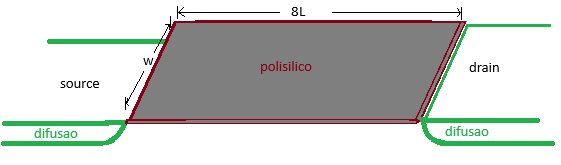
\includegraphics[width=\textwidth]{Transistor8L.png}
        \caption{Transistor A ($L_A = 8L, W_A = W$)}
    \end{minipage}\hfill
    \begin{minipage}{0.45\textwidth}
        \centering
        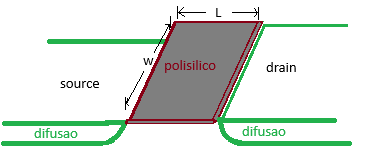
\includegraphics[width=\textwidth]{Transistor1L.png}
        \caption{Transistor B ($L_B = L, W_B = W$)}
    \end{minipage}
\end{figure}

\end{document}